\chapter{Beam Use Proposal}
\label{chap:beam_use_proposal}

\section{Overview}

In this Section we detail the sPHENIX beam use proposal as requested in the ALD Charge (see Appendix~\ref{chap:charge}) for three years of running 2023-2025 assuming 24 or 28 cryo-weeks in each year.   In addition, we provide details on a potential additional two years of running in 2026-2027 that presents a further return on investment in sPHENIX and also the entire RHIC program.   We highlight that this represents the last opportunity for data taking in heavy-ion mode in this energy regime in our lifetime. 

Here we provide a summary of the sPHENIX beam use proposal, following by 
(1) details on C-AD luminosity inputs, (2) experimental commissioning time and ramp up.

ALL THESE NUMBERS ARE JUST PLACEHOLDERS...

%\hline

JUST INCLUDE THE LATEST AUAU HERE....

\begin{table}[h]
\centering
\caption{Summary of Au+Au at 200 GeV option sPHENIX Beam Use Proposal.
The recorded luminosity (Rec. Lum.) and first sampled luminosity (Samp. Lum.) values are for collisions with z-vertex $|z|<$ 10 cm.  The final column shows the sampled luminosity for all z-vertex values, relevant for calorimeter only measurements.\label{tab:summary}}
\bigskip
\centering
\begin{tabular}{ | c | c | c | c | c | c | c | c | }
\hline
Year & Species & $\sqrt{s_{NN}}$ & Cyro  & Physics & Rec. Lum. & Samp. Lum. & Samp. Lum. \\
     &         & [GeV]           & Weeks & Weeks   & $|z|<$10~cm & $|z|<$10~cm & All z-vertex \\ \hline \hline

2023 & \auau   & 200 & 24 (28) & 9 (13) & 3.7 (5.7) \nb   & 4.5 (6.9) \nb & irrelevant \nb \\ \hline
2025 & \auau   & 200 & 24 (28) & 20.5 (24.5) & 13 (15) \nb   & 21 (25) \nb & irrelevant \nb \\ \hline
2027 & \auau   & 200 & 28 & 24.5 & 30 \nb (Demux/Stream)   & 31 \nb & irrelevant \nb \\ \hline
%Year-4 & \pp     & 200          & 23.5          & ---           & 149 \pb & 783 \pb \\ \hline \hline
%Year-5 & \auau   & 200          & 23.5          & 14 \nb   & 48 \nb & 92 \nb \\ \hline
\end{tabular}
\end{table}

\begin{figure}
    \centering
    \includegraphics[width=0.75\linewidth]{figs/figure_sphenix_auaustore.png}
    \caption{Caption}
    \label{fig:sphenixauaustore}
\end{figure}


%\hline


\begin{table}[h]
\centering
\caption{Three-year 2023-2025 sPHENIX Beam Use Proposal.
The recorded luminosity (Rec. Lum.) and first sampled luminosity (Samp. Lum.) values are for collisions with z-vertex $|z|<$ 10 cm.  The final column shows the sampled luminosity for all z-vertex values, relevant for calorimeter only measurements.\label{tab:summary}}
\bigskip
\centering
\begin{tabular}{ | c | c | c | c | c | c | c | c | }
\hline
Year & Species & $\sqrt{s_{NN}}$ & Cyro  & Physics & Rec. Lum. & Samp. Lum. & Samp. Lum. \\
     &         & [GeV]           & Weeks & Weeks   & $|z|<$10~cm & $|z|<$10~cm & All z-vertex \\ \hline \hline

2024 & \pp     & 200 & 24 (28) & 12 (16) & 0.3 (0.4) or 10\% str 7.3 (10.1) & 73 (101) \pb & very little \\ \hline
 --  & \pau    & 200 & --       & 0.003 & 10\% str 0.01 \pb          & 0.11 \pb & very little \\ \hline \hline
%Year-4 & \pp     & 200          & 23.5          & ---           & 149 \pb & 783 \pb \\ \hline \hline
%Year-5 & \auau   & 200          & 23.5          & 14 \nb   & 48 \nb & 92 \nb \\ \hline
\end{tabular}
\end{table}

\begin{table}[h]
\centering
\caption{Two additional years 2026-2027 sPHENIX Beam Use Proposal.
The recorded luminosity (Rec. Lum.) and first sampled luminosity (Samp. Lum.) values are for collisions with z-vertex $|z|<$ 10 cm.  The final column shows the sampled luminosity for all z-vertex values, relevant for calorimeter only measurements.\label{tab:summary}}
\bigskip
\centering
\begin{tabular}{ | c | c | c | c | c | c | c | c | }
\hline
Year & Species & $\sqrt{s_{NN}}$ & Cyro  & Physics & Rec. Lum. & Samp. Lum. & Samp. Lum. \\
     &         & [GeV]           & Weeks & Weeks   & $|z|<$10~cm & $|z|<$10~cm & All z-vertex \\ \hline \hline

2026 & \pp   & 200 & 28 & 15.5      & 0.5 or 100\% str 130~\pb   & 130 \pb & very little \\ \hline
 --  & O+O    & 200 & -- & 2        & 13B + 100\% str 42B & 42B & very little \\ \hline
 --  & Ar+Ar   & 200 & -- & 2.      & 13B + 100\% str 29B & 29B & very little \\ \hline
  2027 & \auau & 200 & 28 & XYZ     & --              & 48 \pb & 267 \pb \\ \hline
%Year-4 & \pp     & 200          & 23.5          & ---           & 149 \pb & 783 \pb \\ \hline \hline
%Year-5 & \auau   & 200          & 23.5          & 14 \nb   & 48 \nb & 92 \nb \\ \hline
\end{tabular}
\end{table}



\begin{table}[h]
\caption{Summary of integrated samples summed for the entire five-year scenario.\label{tab:summary2}}
\bigskip
\centering
\begin{tabular}{ | c | c | c | c | c | c | c | c | c |}
\hline
Species & Energy [GeV] & Rec. Lum. & Samp. Lum. & Samp. Lum. All-Z\\ \hline
\auau   & 200           & 35 \nb (239 billion)  & 80 \nb (550 billion) & 214 \nb (1.5 trillion) \\ \hline 
\pp     & 200          & ---           & 197 \pb (8.3 trillion) & 1.0 \fb (44 trillion) \\ \hline
\pau    & 200          & ---           & 0.33 \pb (0.6 trillion) & 1.46 \pb (2.6 trillion) \\ \hline \hline
\end{tabular}
\end{table}

In the \auau at 200 GeV case, the physics will predominately come from recording minimum bias collisions.   Some additional physics may be "sampled" with rare event triggers, for
example high \pt direct photons.    To be explicit, in the \auau case, the potential gain in statistics for events within the tight z-vertex cut with selective triggering is 550/239 = 2.3  (just over a factor of two gain).    If one can make useful (still to be demonstrated) physics measurements outside that z-vertex range (e.g. with only calorimeters or with just partial TPC tracking and accounting for additional inner detector support material), and effectively trigger, one can gain an even larger factor of 1500/239 = 6.27 (just over a factor of six).   Of course if these triggers do not have very good rejection, one will use up bandwidth otherwise allocated for minimum bias \auau events.

In the \pp and \pau case, the physics will predominantly come from Level-1 triggered events utilizing photon, electron (e.g. from Upsilon decays), hadron, and
jet triggers.  Thus, the key value is the sampled luminosity.   Note that some observables such as lower \pt hadrons (from D, B decays) will likely not sample the full luminosity.  Calorimeter only measurements may utilize most of the z-vertex range for rare probes such as high \pt direct photons and jets.

For \auau minimum bias events, the average number of binary collisions is 
$\left< N_{coll} \right> \approx 250$.  Thus, for hard processes the 239 billion \auau events recorded within $|z|<10$ cm have a rough equivalence in statistics to 59 trillion \pp events.  Similarly, for \pau the $\left< N_{coll} \right> = 4.7$, and thus for hard processes the 0.6 trillion \pau events have a rough equivalence in statistics to 2.8 trillion \pp events.   Note of course that for the \auau sample, analyses will divide the data into centrality selections.

\section{RHIC Luminosity Projections}

For planning purposes in this document, we use luminosity projection numbers provided by the Collider-Accelerator Division (C-AD).   The version of the document titled 
"RHIC Collider Projections (FY 2017 –- FY 2027)" utilized for this study is dated 12 May 2017 and utilizes knowledge gained from the Run-15 \pp and \pau at 200 GeV running and the Run-16 \auau at 200 GeV running.   The document is available at:

\bigskip
{\color{blue}{http://www.rhichome.bnl.gov/RHIC/Runs/RhicProjections.pdf}} 
\bigskip

Note that the document linked above is periodically updated, so note the date tag.  In general, C-AD provides a minimum and maximum luminosity per week for each running period, as well as the fraction of collisions within a given z-vertex range. For calculating the integrated luminosity, we assume a ramp-up curve and then a steady-state physics running at the mean of the minimum and maximum in both luminosity and z-vertex fraction $f_{z}$ (where a minimum and maximum are given).   

\subsection{Vertex Range}

For this sPHENIX set of calculations, we consider the z-vertex range -10 cm $< z < $ + 10 cm, referred to as $f_{z10}$, i.e. the narrow vertex range.
The $f_{z10}$ values decrease during the course of a store due to broadening of the bunches.   This modest effect is not taken into account in these calculations.

With the MAPS inner tracker as detailed in the MVTX pre-proposal, the active ladder length is 271.2 mm or $\pm$135.6 mm.  The layers are at $R_1$ = [22.4-26.7] mm, $R_2$ = [30.1-34.6] mm, and $R_3$ = [37.8-42.1] mm [see Table 2 of the MVTX pre-proposal]. Therefore, collisions taking place with $\pm 10$ cm will have acceptance of $|\eta| \le$ 1.0 if one requires all tracks in this $\eta$ range to pass through at least two layers of MAPS.    We may also quote values for all z-vertices $f_{zall}=1$, and these events are potentially useful for calorimeter only measurements (for example inclusive direct photons and photon-jet correlations).   

At this point, we do not include effects from the z-vertex resolution of the sPHENIX minimum bias (MB) trigger detector in being able to select specifically events within the $\pm 10$ cm range.    We expect an approximate resolution of $\sigma \approx 0.5-1.0$ cm in \auau collisions at 200 GeV.    We also highlight that the tracking has a somewhat larger z-vertex collision coverage that can be utilized, just without the same $|\eta| \le$ 1.0 coverage.

\subsection{Ramp-Up Assumptions}

For mapping out a run plan, we state both cryo-weeks for a running period and also physics data taking weeks, i.e. when Physics Running is declared by C-AD.   The guidance from C-AD is that there is a 0.5 week "cool down from 50 K to 4 K", then a 2.0 week "set-up mode" for the specific collision species, and then a 0.5 week "ramp-up".   If switching species, there is again a 2.0 week "set-up" and 0.5 week "ramp-up".    Lastly, at the end of the running period, there is a 0.5 "warm-up from 4 K to 50 K".  

In addition, we assume that in the first, second and third weeks of declared Physics Running, one achieves 25\%, 50\%, and then 75\% of the luminosity target, with subsequent weeks at 100\% (again of the mean of the minimum and maximum).

\subsection{Summary of C-AD Numbers}

Here are the basic inputs for the three collisions systems considered in this sPHENIX run plan (\pp, \pau, \auau all at 200 GeV).

\subsubsection{\auau at 200 GeV}

The C-AD projections are summarized in their document, Table 4.   We 
reproduce some of those key values here in Table~\ref{tab:auauspecs}.  

\begin{table}[h]
\centering
\caption{Summary of C-AD key values for \auau at 200 GeV running with the year labels as given in the C-AD document.
\label{tab:auauspecs}}
\bigskip
\begin{tabular}{ | c | c | c | c | c | c | c | c |}
\hline
Mode & \nb/wk & \nb/wk & $f_{z10}$ & $f_{z10}$ & ave/peak & peak rate & peak rate $\times f_{z10}$ \\ 
   	 & [min] & [max] & [min] & [max] &  & [max] & [max] \\ \hline
	Au+Au~(2022E) & 3 & 4.75 & 0.19 & 0.3 & 0.6 & 1.5E5 & 4.5E4 \\ \hline
	Au+Au~(2024E) & 3 & 7.02 & 0.3 & 0.3 & 0.6  & 2.2E5 & 6.6E4  \\ \hline
	Au+Au~(2026E) & 3 & 7.51 & 0.3 & 0.3 & 0.6  & 2.4E5 & 7.1E4  \\ \hline 
\end{tabular}
\end{table}

We consider running \auau in three calendar years (Year-1, Year-3, Year-5).   For the Year-1 run, we utilize the C-AD values they label as {\bf{2022E}}, where the minimum values correspond to those achieved in the 2016 run and the maximum are 58\% higher.   Wolfram Fischer has provided us with Figure~\ref{fig:auaustore} showing an example "best store" from Run-16 \auau at 200 GeV, where "best" is actually one of many stores that were reproduced with the same settings.  
The $f_{z10} = 0.19$ from Run-16 \auau is used as the minimum value, and 
$f_{z10} = 0.30$ is the projected maximum value.

\begin{figure}
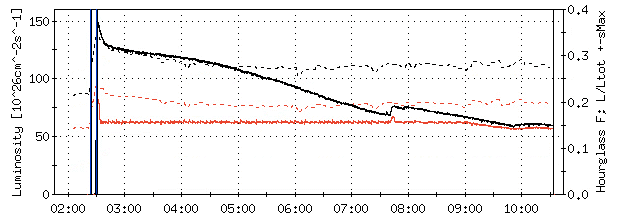
\includegraphics[]{figure_cad_run16auau_examplestore}
\caption{Run-16 \auau at 200 GeV store.   The black line shows the luminosity (left y-axis units) as a function of time in store in hours.   The red dashed line shows the fraction of collisions within $\pm$ 10 cm. \label{fig:auaustore}}
\end{figure}

\subsubsection{\pp at 200 GeV}

The C-AD projections are summarized in their document, Table 6.   We 
reproduce some of those key values here in Table~\ref{tab:ppspecs}.  
Wolfram Fischer has provided us with Figure~\ref{fig:auaustore} showing an example "best store" from Run-15 \pp at 200 GeV, where "best" is actually one of many stores that were reproduced with the same settings.  

\begin{table}[h]
\centering
\caption{Summary of C-AD key values for \pp at 200 GeV running.
\label{tab:ppspecs}}
\bigskip
\begin{tabular}{ | c | c | c | c | c | c | c | c |}
\hline
Mode & \pb/wk & \pb/wk & $f_{z10}$ & $f_{z10}$ & ave/peak & peak rate & peak rate $\times f_{z10}$ \\ 
   	 & [min] & [max] & [min] & [max] &  & [max] & [max] \\ \hline
	p+p~(2023E) & 25 & 64 & 0.16 & 0.19 & 0.6 & 1.2E7 & 2.4E6 \\ \hline
	p+p~(2025E) & 25 & 64 & 0.19 & 0.19 & 0.6  & 1.2E7 & 2.4E6  \\ \hline
\end{tabular}
\end{table}

\begin{figure}
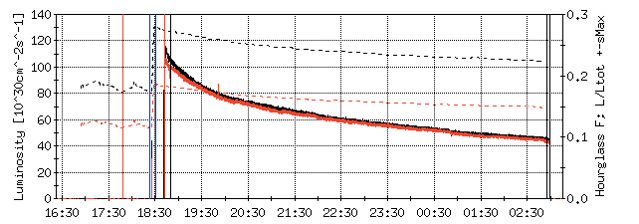
\includegraphics[]{figure_cad_run15pp200_examplestore}
\caption{Run-15 \pp at 200 GeV store.   The black line shows the luminosity (left y-axis units) as a function of time in store in hours.   The red dashed line shows the fraction of collisions within $\pm$ 10 cm.}
\end{figure}

\subsubsection{\pau at 200 GeV}

The C-AD projections are summarized in their document, Table 8.   We 
reproduce some of those key values here in Table~\ref{tab:pauspecs}.    

\begin{table}[h]
\centering
\caption{Summary of C-AD key values for \pau at 200 GeV running.
\label{tab:pauspecs}}
\bigskip
\begin{tabular}{ | c | c | c | c | c | c | c | c |}
\hline
Mode & \pb/wk & \pb/wk & $f_{z10}$ & $f_{z10}$ & ave/peak & peak rate & peak rate $\times f_{z10}$ \\ 
   	 & [min] & [max] & [min] & [max] &  & [max] & [max] \\ \hline
	p+Au~(2023E) & 0.14 & 0.35 & 0.17 & 0.25 & 0.6 & 2.8E6 & 6.9E5 \\ \hline
\end{tabular}
\end{table}

\section{5-Year sPHENIX Run Plan}

For this plan, we assume an sPHENIX uptime (i.e. the fraction of time when collisions are available that sPHENIX is taking data with high livetime) of 0.60 for the first two years of running (Year-1 and Year-2) since the detector is being commissioned and new Level-1 triggers are being brought online, and 0.80 for the subsequent runs Years-3,4,5.  These uptime value fold in the expected deadtime of the data acquisition system - of order 90-95\%.
Note that the first year of running also includes substantial additional commissioning time, not included in the physics data taking segment.

RHIC C-AD projections for time in store (i.e. RHIC uptime) vary slightly with most of the projected values around 0.60.   Thus, we will use this single value for all cases.  It is notable that C-AD projections are for a nominal 8 hour store; however, a more optimal store length may be found in future running at closer to 5 hours.

\subsection{\auau at 200 GeV}

For the first sPHENIX run in Year-1 with \auau at 200 GeV collisions, we plan on 30 cryo-weeks as detailed in Table~\ref{tab:cryoplan2022}.  Significant commissioning time is included in the run plan.   Again note that in addition to the specifically called out "Initial Commission Time" and assumed sPHENIX uptime is 60\% for the first two runs.

\begin{table}
\centering
\begin{tabular}{ | c | l | }
\hline
Weeks & Designation \\ \hline
0.5  & Cool Down from 50 K to 4 K \\ \hline
2.0  & Set-up mode 1 (Au+Au at 200 GeV) \\ \hline
0.5  & Ramp-up mode 1 (8 h/night for experiments) \\ \hline
11.5  & sPHENIX Initial Commission Time \\ \hline
9.0 & Data taking mode 1 (Physics) \\ \hline
0.5  & Controlled refrigeration turn-off \\ \hline \hline \hline
24.0 & Total cryo-weeks \\
\hline
\end{tabular}
\caption{Example cryo-week run plan for the first sPHENIX run in Year-1 with \auau at 200 GeV collisions.\label{tab:cryoplan2022}}
\end{table}

\begin{table}
\centering
\begin{tabular}{ | c | l | }
\hline
Weeks & Designation \\ \hline
0.5  & Cool Down from 50 K to 4 K \\ \hline
2.0  & Set-up mode 1 (Au+Au at 200 GeV) \\ \hline
0.5  & Ramp-up mode 1 (8 h/night for experiments) \\ \hline
24.5 & Data taking mode 1 (Physics) \\ \hline
0.5  & Controlled refrigeration turn-off \\ \hline \hline \hline
28.0 & Total cryo-weeks \\
\hline
\end{tabular}
\caption{Example cryo-week run plan for the first sPHENIX run in 2027 with \auau at 200 GeV collisions.\label{tab:cryoplan2022}}
\end{table}

Subsequent \auau at 200 GeV runs (Year-3 and Year-5) have 23.5 weeks of Physics Data Taking are no additional commissioning time - thus adding up to a total of 27 cryo-weeks each.   

\begin{table}
\centering
\begin{tabular}{ | c | l | }
\hline
Weeks & Designation \\ \hline
0.5  & Cool Down from 50 K to 4 K \\ \hline
2.0  & Set-up mode 1 (Au+Au at 200 GeV) \\ \hline
0.5  & Ramp-up mode 1 (8 h/night for experiments) \\ \hline
20.5 & Data taking mode 1 (Physics) \\ \hline
0.5  & Controlled refrigeration turn-off \\ \hline \hline \hline
24.0 & Total cryo-weeks \\
\hline
\end{tabular}
\caption{Example cryo-week run plan for the first sPHENIX run in Year-3 with \auau at 200 GeV collisions.\label{tab:cryoplan2022}}
\end{table}

A useful number for \auau at 200 GeV collisions assuming a 6.8 barn inelastic cross section is that $1 nb^{-1} = 6.8 \times 10^{9}$ events.    Thus, the recorded event sets of 7, 14, and 14 $1 nb^{-1}$ for the runs in 2022, 2024, and 2026 respectively, correspond to 47, 96, and 96 billion events.   The 
key requirements to achieve these recorded event sets are (1) the sPHENIX Data Acquisition Level-1 accept rate of 15 kHz with livetime from 90-95\%, (2) the luminosity corresponds to a rate of collisions within $|z|<$10 cm during the store above 15 kHz, and (3) maintaining the sPHENIX and RHIC uptime projections.  Figure~\ref{fig:auaulumcurves} shows the \auau collision rate as a function of time in store in hours for the three years of projected running both with and without the z-vertex cut.   This indicates that condition (2) above is satisfied.

\begin{figure}
\centering
%\includegraphics[max size={0.85\textwidth}]{figure_sphenix_auau200ratesvstime}
\includegraphics[width=0.85\linewidth]{figure_sphenix_auaustore} % I think this is the correct file name.  DPM
\caption{Estimated \auau at 200 GeV collision rate as a function of time in store for all collisions (blue) and collisions within $\pm$ 10 cm (red).  The bottom to top set of curves in each color are for the mean luminosity and $f_{z10}$ for the C-AD projections labeled in their document as 2022E, 2024E, 2026E and corresponding to sPHENIX running in Year-1, Year-3, and Year-5.   Also shown as a green band is the sPHENIX DAQ Rate of 15 kHz for reference.
\label{fig:auaulumcurves}}
\end{figure}

\subsection{\pp and \pau at 200 GeV}

The run in Year-2 is projected to be split between \pp and \pau at 200 GeV 
with the cryo-week plan shown in Table~\ref{tab:cryo2023}.

\begin{table}
\centering
\begin{tabular}{ | c | l | }
\hline
Weeks & Designation \\ \hline
0.5  & Cool Down from 50 K to 4 K \\ \hline
2.0  & Set-up mode 1 (p+p at 200 GeV) \\ \hline
0.5  & Ramp-up mode 1 (8 h/night for experiments) \\ \hline
12.0 & Data taking mode 1 (p+p Physics) \\ \hline
1.0  & Move DX magnets \\ \hline
2.0  & Set-up mode 2 (p+Au at 200 GeV) \\ \hline
0.5  & Ramp-up mode 2 (8 h/night for experiments) \\ \hline
5.0 & Data taking mode 2 (p+Au Physics) \\ \hline
0.5  & Controlled refrigeration turn-off \\ \hline \hline \hline
24.0 & Total cryo-weeks \\
\hline
\end{tabular}
\caption{Example cryo-week run plan for Year-2.\label{tab:cryo2023}}
\end{table}

Note that for all the luminosity projections and conversions to collision rates we utilize as total inelastic cross sections: 
6.8 barns, 1.7 barns, 42 millibarns for \auau, \pau, and \pp respectively.

\begin{table}
\centering
\begin{tabular}{ | c | l | }
\hline
Weeks & Designation \\ \hline
0.5  & Cool Down from 50 K to 4 K \\ \hline
2.0  & Set-up mode 1 (p+p at 200 GeV) \\ \hline
0.5  & Ramp-up mode 1 (8 h/night for experiment) \\ \hline
15.5 & Data taking mode 1 (p+p Physics) \\ \hline
2.0  & Set-up mode 2 (O+O at 200 GeV) \\ \hline
0.5  & Ramp-up mode 2 (8 h/night for experiment) \\ \hline
2.0 & Data taking mode 2 (O+O Physics) \\ \hline
2.0  & Set-up mode 3 (Ar+Ar at 200 GeV) \\ \hline
0.5  & Ramp-up mode 3 (8 h/night for experiment) \\ \hline
2.0 & Data taking mode 3 (Ar+Ar Physics) \\ \hline
0.5  & Controlled refrigeration turn-off \\ \hline \hline \hline
28.0 & Total cryo-weeks \\
\hline
\end{tabular}
\caption{Example cryo-week run plan for Year-4.\label{tab:cryo2023}}
\end{table}

\section{Charge Particle Flux}

The inner tracking detectors have performance issues related to the total charge particle flux - i.e. the number of charged particle tracks per unit pseudorapidity per unit time.   The Time Projection Chamber in particular will have space charge distortions that are related to exactly this quantity - i.e. $dN_{ch}/d\eta/$second.   In Table~\ref{tab:chargerates}, we show the estimated midrapidity $dN_{ch}/d\eta$, the maximum projected peak collision rate (over all vertices since they all contribute charge in the detector), and the figure of merit $dN_{ch}/d\eta/$second.

\begin{table}[h]
\centering
\caption{Charged particle instantaneous rate (max).  These values are the maximum projected values during the five-year run plan and are from collisions over all z-vertex values.\label{tab:chargerates}}
\bigskip
\begin{tabular}{ | c | c | c | c | c |}
\hline
System & Energy & $dN_{ch}/d\eta$ & Highest Rate & $dN_{ch}/d\eta$/second \\ \hline \hline
p+p & 200 GeV & 2.29 & 12.9 MHz & $28 \times 10^{6}$ \\ \hline
p+Au & 200 GeV & 9.16 & 2.8 MHz & $29 \times 10^{6}$ \\ \hline
Au+Au & 200 GeV & 190 & 219 kHz & $45 \times 10^{6}$ \\ \hline
\end{tabular}
\end{table}

\section{Radiation Dose}

There are other detectors that are sensitive to the total integrated charged particle production over all running periods.   These are related to things like radiation damage or degradation - for example the SiPMs.   Note that radiation exposure can be related to beam-scrape, beam-loss events, which are not accounted for here.   The results below give a quantity that should be proportional to the collision related radiation exposure.

Table~\ref{tab:radiation} gives values for the estimated total charged particle exposure per unit pseudorapidity.

\begin{table}[h]
\centering
\caption{Scaling with radiation dose (collision related only).  The Integrated Charge Particles represents the total number of charged particles per unit pseudo-rapidity in all collisions during the running period.  These are maximum values.  The values listed for Run-15 \pp and Run-14 \auau are very rough estimates given the length of the runs and the high value luminosities.\label{tab:radiation}}
\bigskip
\begin{tabular}{|c | c | c | c| c|}
\hline
System & Energy & $dN_{ch}/d\eta$ & Run & Integrated Charged Particles \\ \hline \hline
p+p & 200 GeV & 2.29 & Run-15 & 2.5E13 \\ \hline
p+p & 200 GeV & 2.29 & 2023 & 3.7E13 \\ \hline
p+p & 200 GeV & 2.29 & 2025 & 11.0E13 \\ \hline \hline
p+Au & 200 GeV & 9.16 & 2023 & 3.2E13 \\ \hline \hline
Au+Au & 200 GeV & 190 & Run-16 & 2.7E13 \\ \hline
Au+Au & 200 GeV & 190 & 2022 & 5.3E13 \\ \hline
Au+Au & 200 GeV & 190 & 2024 & 16.0E13 \\ \hline
Au+Au & 200 GeV & 190 & 2026 & 17.0E13 \\ \hline \hline
\end{tabular}
\end{table}

\section{Trigger Requirements}

In particular for the physics program in \pp and \pau selective Level-1 triggers are required to sample the full luminosity.   Triggering using the EMCal for single photons (typically with \pt greater than 10 Gev/c) and for electrons (from Upsilon decays typically with \pt greater than 3-4 GeV/c) are in development.  In addition, triggering using the combined EMCal and HCal are needed for selected jets and single hadrons.    At the highest \pp interaction rates, rejection factors of order 5000-10,000 are needed to result in a 1-2 kHz bandwidth allocation.    A separate note will detail the Level-1 trigger projected performance. 

More challenging will be extracting additional physics in \auau collisions beyond the recorded minimum bias sample.   It might be reasonable to reduce the 15 kHz minimum bias archiving rate by 1-2 kHz in order to free up bandwidth to sample the full luminosity for a few rare triggers.   For example, sampling the full \auau luminosity for single photons with \pt greater than 15 GeV/c should require very modest bandwidth.   Sampling additional luminosity for the highest \pt jets or Upsilons decays (perhaps in peripheral events only) will be more challenging.
